%HW5.tex
%
% Fifth Homework for Graduate Algebra
% Frank Sottile
%%%%%%%%%%%%%%%%%%%%%%%%%%%%%%%%%%%%%%%%%%%%%%%%%%%%%%%%%%%%%%%%%%%%%%%
\documentclass[12pt]{article}
\usepackage{multicol,amssymb,amsmath}
\usepackage{graphicx}
\usepackage{xcolor}
\headheight=8pt
%
\topmargin=-95pt
\textheight=744pt   \textwidth=575pt
\oddsidemargin=-60pt \evensidemargin=-60pt

\pagestyle{empty}

%%%%%%%%%%%%%%%%%%%%%%%%%%%%%%%%%%%%%%%%%%%%
\newcommand{\HH}{{\mathbb H}}
\newcommand{\FF}{{\mathbb F}}
\newcommand{\RR}{{\mathbb R}}
\newcommand{\CC}{{\mathbb C}}
\newcommand{\KK}{{\mathbb K}}
\newcommand{\NN}{{\mathbb N}}
\newcommand{\QQ}{{\mathbb Q}}
\newcommand{\TT}{{\mathbb T}}
\newcommand{\ZZ}{{\mathbb Z}}
\newcommand{\calA}{{\mathcal A}}
\newcommand{\be}{{\bf e}}

\newcommand{\Hom}{\mbox{Hom}}
\newcommand{\End}{\mbox{End}}
\newcommand{\Mat}{\mbox{Mat}}
\newcommand{\rank}{\mbox{rank}}
\newcommand{\spec}{\mbox{spec}}
\newcommand{\cone}{\mbox{cone}}

\newcommand{\Square}{\raisebox{-2pt}{\includegraphics{figures/Square.eps}}}

\newcommand{\vect}[2]{(\begin{smallmatrix}#1\\#2\end{smallmatrix})}
\newcommand{\msp}{\hspace{8pt}}

\newcommand{\barsl}{\noindent\begin{minipage}[t]{575pt}
{\color{violet}\rule{575pt}{1.2pt}}\vspace{-5.7mm}\\
{\color{blue}\rule{575pt}{1.2pt}}\vspace{-5.7mm}\\
{\color{green}\rule{575pt}{1.2pt}}\vspace{-5.7mm}\\
{\color{yellow}\rule{575pt}{1.2pt}}\vspace{-5.7mm}\\
{\color{orange}\rule{575pt}{1.2pt}}\vspace{-5.7mm}\\
{\color{red}\rule{575pt}{1.2pt}}
\end{minipage}}


\def\demph#1{{\color{blue}{\sl #1}}}
\def\defcolor#1{{\color{blue}#1}}

\begin{document}
\LARGE 
\noindent
Algebra II\ \ Winter 2021 \hfill 15 February\makebox[40pt][l]{\ }\newline
Frank Sottile \hfill
\Large\sf
Fifth Homework\makebox[40pt][l]{\ }
\vspace{5pt}
\normalsize

\noindent
Write your answers neatly, in complete sentences, and prove all assertions.
Start each problem on a new page (this makes it easier in Gradescope).
Revise your work before handing it in, and submit a .pdf  created from a LaTeX source to Gradescope.
Correct and crisp proofs are greatly appreciated; oftentimes your work can be shortened and made clearer.

\noindent
{\color{red}Due Monday 22 February.}\vspace{1pt}

\barsl

\begin{enumerate}
%%%%%%%%%%%%%%%%%%%%%%%%%%%%%%%%%%%%%
%\setcounter{enumi}{52}

%\newpage
%%%%%%%%%%%%%%%%%%%%%%%%%%%%%%%%%%%%%%%%%%%%%%%%%%%%%%%%%%%%%%%%%%%%%%%%%%%%%%%%%
 \item  Recall that $\ZZ_2=\ZZ/2\ZZ$ is the group of integers modulo 2.
 Let $\pi\colon \ZZ\to\ZZ_2$ be the canonical surjection.
 Prove that the induced map $\pi_*\colon\Hom_\ZZ(\ZZ_2,\ZZ)\to\Hom_\ZZ(\ZZ_2,\ZZ_2)$ is the zero map and is therefore not a surjection.
 (You could do worse than compute all the $\Hom$-groups.)
 \vspace{-2pt}
%%%%%%%%%%%%%%%%%%%%%%%%%%%%%%%%%%%%%%%%%%%%%%%%%%%%%%%%%%%%%%%%%%%%%%%%%%%%%%%%%

%\newpage
%%%%%%%%%%%%%%%%%%%%%%%%%%%%%%%%%%%%%%%%%%%%%%%%%%%%%%%%%%%%%%%%%%%%%%%%%%%%%%%%%
\item   For a ring $R$, let \defcolor{$R^{\rm op}$}  be the abelian group $R$ with multiplication
  $\defcolor{\cdot_{\rm op}}\colon R\times R \to R$ define by $s\defcolor{\cdot_{\rm op}r:=rs}$.\newline
  (This is called the \demph{opposite ring to $R$}.)

  Prove that there is a ring isomorphism $\Hom_R(R,R)\xrightarrow{\,\sim\,} R^{\rm op}$.
 \vspace{-2pt} 
%%%%%%%%%%%%%%%%%%%%%%%%%%%%%%%%%%%%%%%%%%%%%%%%%%%%%%%%%%%%%%%%%%%%%%%%%%%%%%%%%


%\newpage
%%%%%%%%%%%%%%%%%%%%%%%%%%%%%%%%%%%%%%%%%%%%%%%%%%%%%%%%%%%%%%%%%%%%%%%%%%%%%%%%%
\item  Write carefully the proof that the following conditions on a module $J$ over a ring $R$ are equivalent:
  \begin{enumerate}
  \item $J$ is injective.
  \item If $\varphi\colon A\to B$ an injection of $R$-modules, then
    $\varphi^*\colon\Hom_R(B,J)\to\Hom_R(A,J)$ is a surjection of abelian groups.
  \item  The functor $\Hom_R(-,J)$ from $R$-modules to abelian groups is an exact functor.
  \end{enumerate}
   \vspace{-2pt}
%%%%%%%%%%%%%%%%%%%%%%%%%%%%%%%%%%%%%%%%%%%%%%%%%%%%%%%%%%%%%%%%%%%%%%%%%%%%%%%%%

\end{enumerate}
%%%%%%%%%%%%%%%%%%%%%%%%%%%%%%%%%%%%%%%%%%%%%%%%%%%%%%%%%%%%%%%


\end{document}

%\newpage
%%%%%%%%%%%%%%%%%%%%%%%%%%%%%%%%%%%%%%%%%%%%%%%%%%%%%%%%%%%%%%%%%%%%%%%%%%%%%%%%%
\item 
   \vspace{-2pt}
%%%%%%%%%%%%%%%%%%%%%%%%%%%%%%%%%%%%%%%%%%%%%%%%%%%%%%%%%%%%%%%%%%%%%%%%%%%%%%%%%

%\newpage
%%%%%%%%%%%%%%%%%%%%%%%%%%%%%%%%%%%%%%%%%%%%%%%%%%%%%%%%%%%%%%%%%%%%%%%%%%%%%%%%%
 \item  For any homomorphism $f\colon A\to B$ of left $R$-modules, prove that the diagram
   \[
    \begin{picture}(80,62)(-5,0)
        \put(  0,50){$A$} \put( 17,54){\vector(1,0){28}}\put(24,58){\small$\theta_A$}  
        \put( 50,50){$A^{**}$} 
 
        \put(  7,45){\vector(0,-1){32}}  \put( -4,30){\small$f$}
        \put( 57,45){\vector(0,-1){32}}  \put( 60,30){\small$f^{**}$}

        \put(  0,0){$B$} \put( 17,4){\vector(1,0){28}} \put(24, 8){\small$\theta_B$}   
        \put( 50,0){$B^{**}$} 
        \end{picture}
 \]
 is commutative.
 Here $\defcolor{\theta_A}\colon A \to A^{**}$ is the natural map from the $A$-module to its second dual, and\newline
 $\defcolor{f^{**}}\colon A^{**}\to B^{**}$ is the double pullback map between second duals.

 Conclude that $\theta$ is a natural transformation from the identity functor on the category of left $R$-modules to the functor $^{**}$ of
 taking second duals.
   \vspace{-2pt}
%%%%%%%%%%%%%%%%%%%%%%%%%%%%%%%%%%%%%%%%%%%%%%%%%%%%%%%%%%%%%%%%%%%%%%%%%%%%%%%%%



%\newpage
%%%%%%%%%%%%%%%%%%%%%%%%%%%%%%%%%%%%%%%%%%%%%%%%%%%%%%%%%%%%%%%%%%%%%%%%%%%%%%%%%
\item  Let $R$ be a ring and $M$ a finitely-generated left $R$-module.
  Recall that $\Hom_R(M,R)$ is a right $R$-module.\newline
  Show that if $M$ is projective, then $\Hom_R(M,R)$ is projective.

  Show that $M$ is a reflexive $R$-module.
   \vspace{-2pt}
%%%%%%%%%%%%%%%%%%%%%%%%%%%%%%%%%%%%%%%%%%%%%%%%%%%%%%%%%%%%%%%%%%%%%%%%%%%%%%%%%


%\newpage
%%%%%%%%%%%%%%%%%%%%%%%%%%%%%%%%%%%%%%%%%%%%%%%%%%%%%%%%%%%%%%%%%%%%%%%%%%%%%%%%%
 \item
   Let $F$ be a free left $R$-module of infinite rank.
   Show that $F$ is not reflexive.
   \vspace{-2pt}
%%%%%%%%%%%%%%%%%%%%%%%%%%%%%%%%%%%%%%%%%%%%%%%%%%%%%%%%%%%%%%%%%%%%%%%%%%%%%%%%%

\end{enumerate}
%%%%%%%%%%%%%%%%%%%%%%%%%%%%%%%%%%%%%%%%%%%%%%%%%%%%%%%%%%%%%%%


\end{document}

%\newpage
%%%%%%%%%%%%%%%%%%%%%%%%%%%%%%%%%%%%%%%%%%%%%%%%%%%%%%%%%%%%%%%%%%%%%%%%%%%%%%%%%
\item 
   \vspace{-2pt}
%%%%%%%%%%%%%%%%%%%%%%%%%%%%%%%%%%%%%%%%%%%%%%%%%%%%%%%%%%%%%%%%%%%%%%%%%%%%%%%%%
